\documentclass{beamer}

% load packages
\usepackage[utf8]{inputenc}
\usepackage{graphicx}	% use graphic path
\usepackage{graphbox}	% needed to align graphics relative to text
%\usepackage[export]{adjustbox}
\usepackage{xcolor}		% needed for colored text
\usepackage{enumitem}	% use "plus" and "minus" symbols as bullets in itemize (pro/con lists)

% setup enumitem in way compatible with beamer
\setitemize{label=\usebeamerfont*{itemize item}%
  \usebeamercolor[fg]{itemize item}
  \usebeamertemplate{itemize item}}

% set directory for the images
\graphicspath{{../images/}}

% setup theme
\usetheme{metropolis}

% title information
\title{Non-contact, automated cardiac pulse measurements using video imaging and blind source separation.}
\author{Ming-Zher Poh, Daniel J. McDuff, Rosalind W. Picard}
\date{2010}

\begin{document}

% own commands
\newcommand{\mytitle}[1]{{\Large{\underline{#1}}}}
\newcommand{\positiveaspect}{\textcolor{green}{$\oplus$}}
\newcommand{\negativeaspect}{\textcolor{red}{$\ominus$}}

% title page
\frame{\titlepage}

% start slides
\begin{frame}{Why to measure the pulse?}
\begin{itemize}
	\item General health indicator \pause
	\item Important for therapy of chronic diseases \pause
	\item Resting heart rate: risk factor of its own\\ \pause
		Comparable to smoking!\\
		
\includegraphics[width=1cm]{No_Smoking} \pause
	\item Scientific long term studies (e.~g. sleep studies)\\
		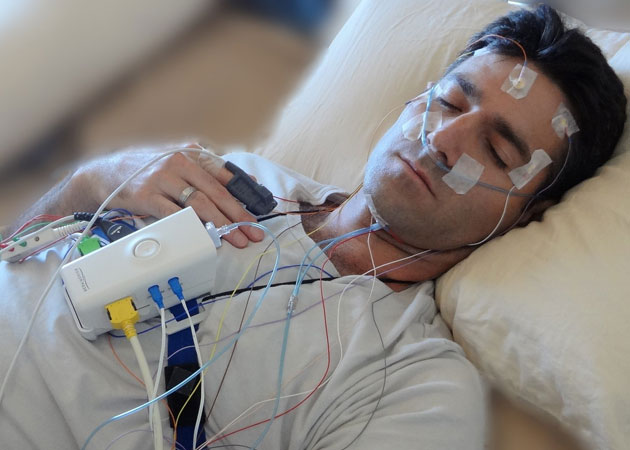
\includegraphics[width=0.4\textwidth]{Sleep-lab-facilities.jpg}
\end{itemize}
\end{frame}

\begin{frame}{Heart rate measurement (Traditional)}
\begin{itemize}
	\item \mytitle{Electrocardiography}\\
		\vspace{0.2cm}
		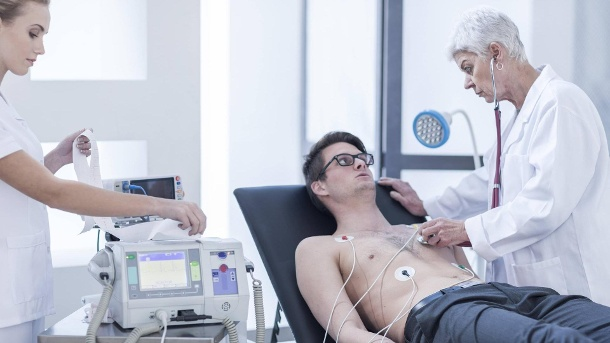
\includegraphics[width=0.45\textwidth, height=0.3\paperheight]{ekg.jpg}
		\hfill
		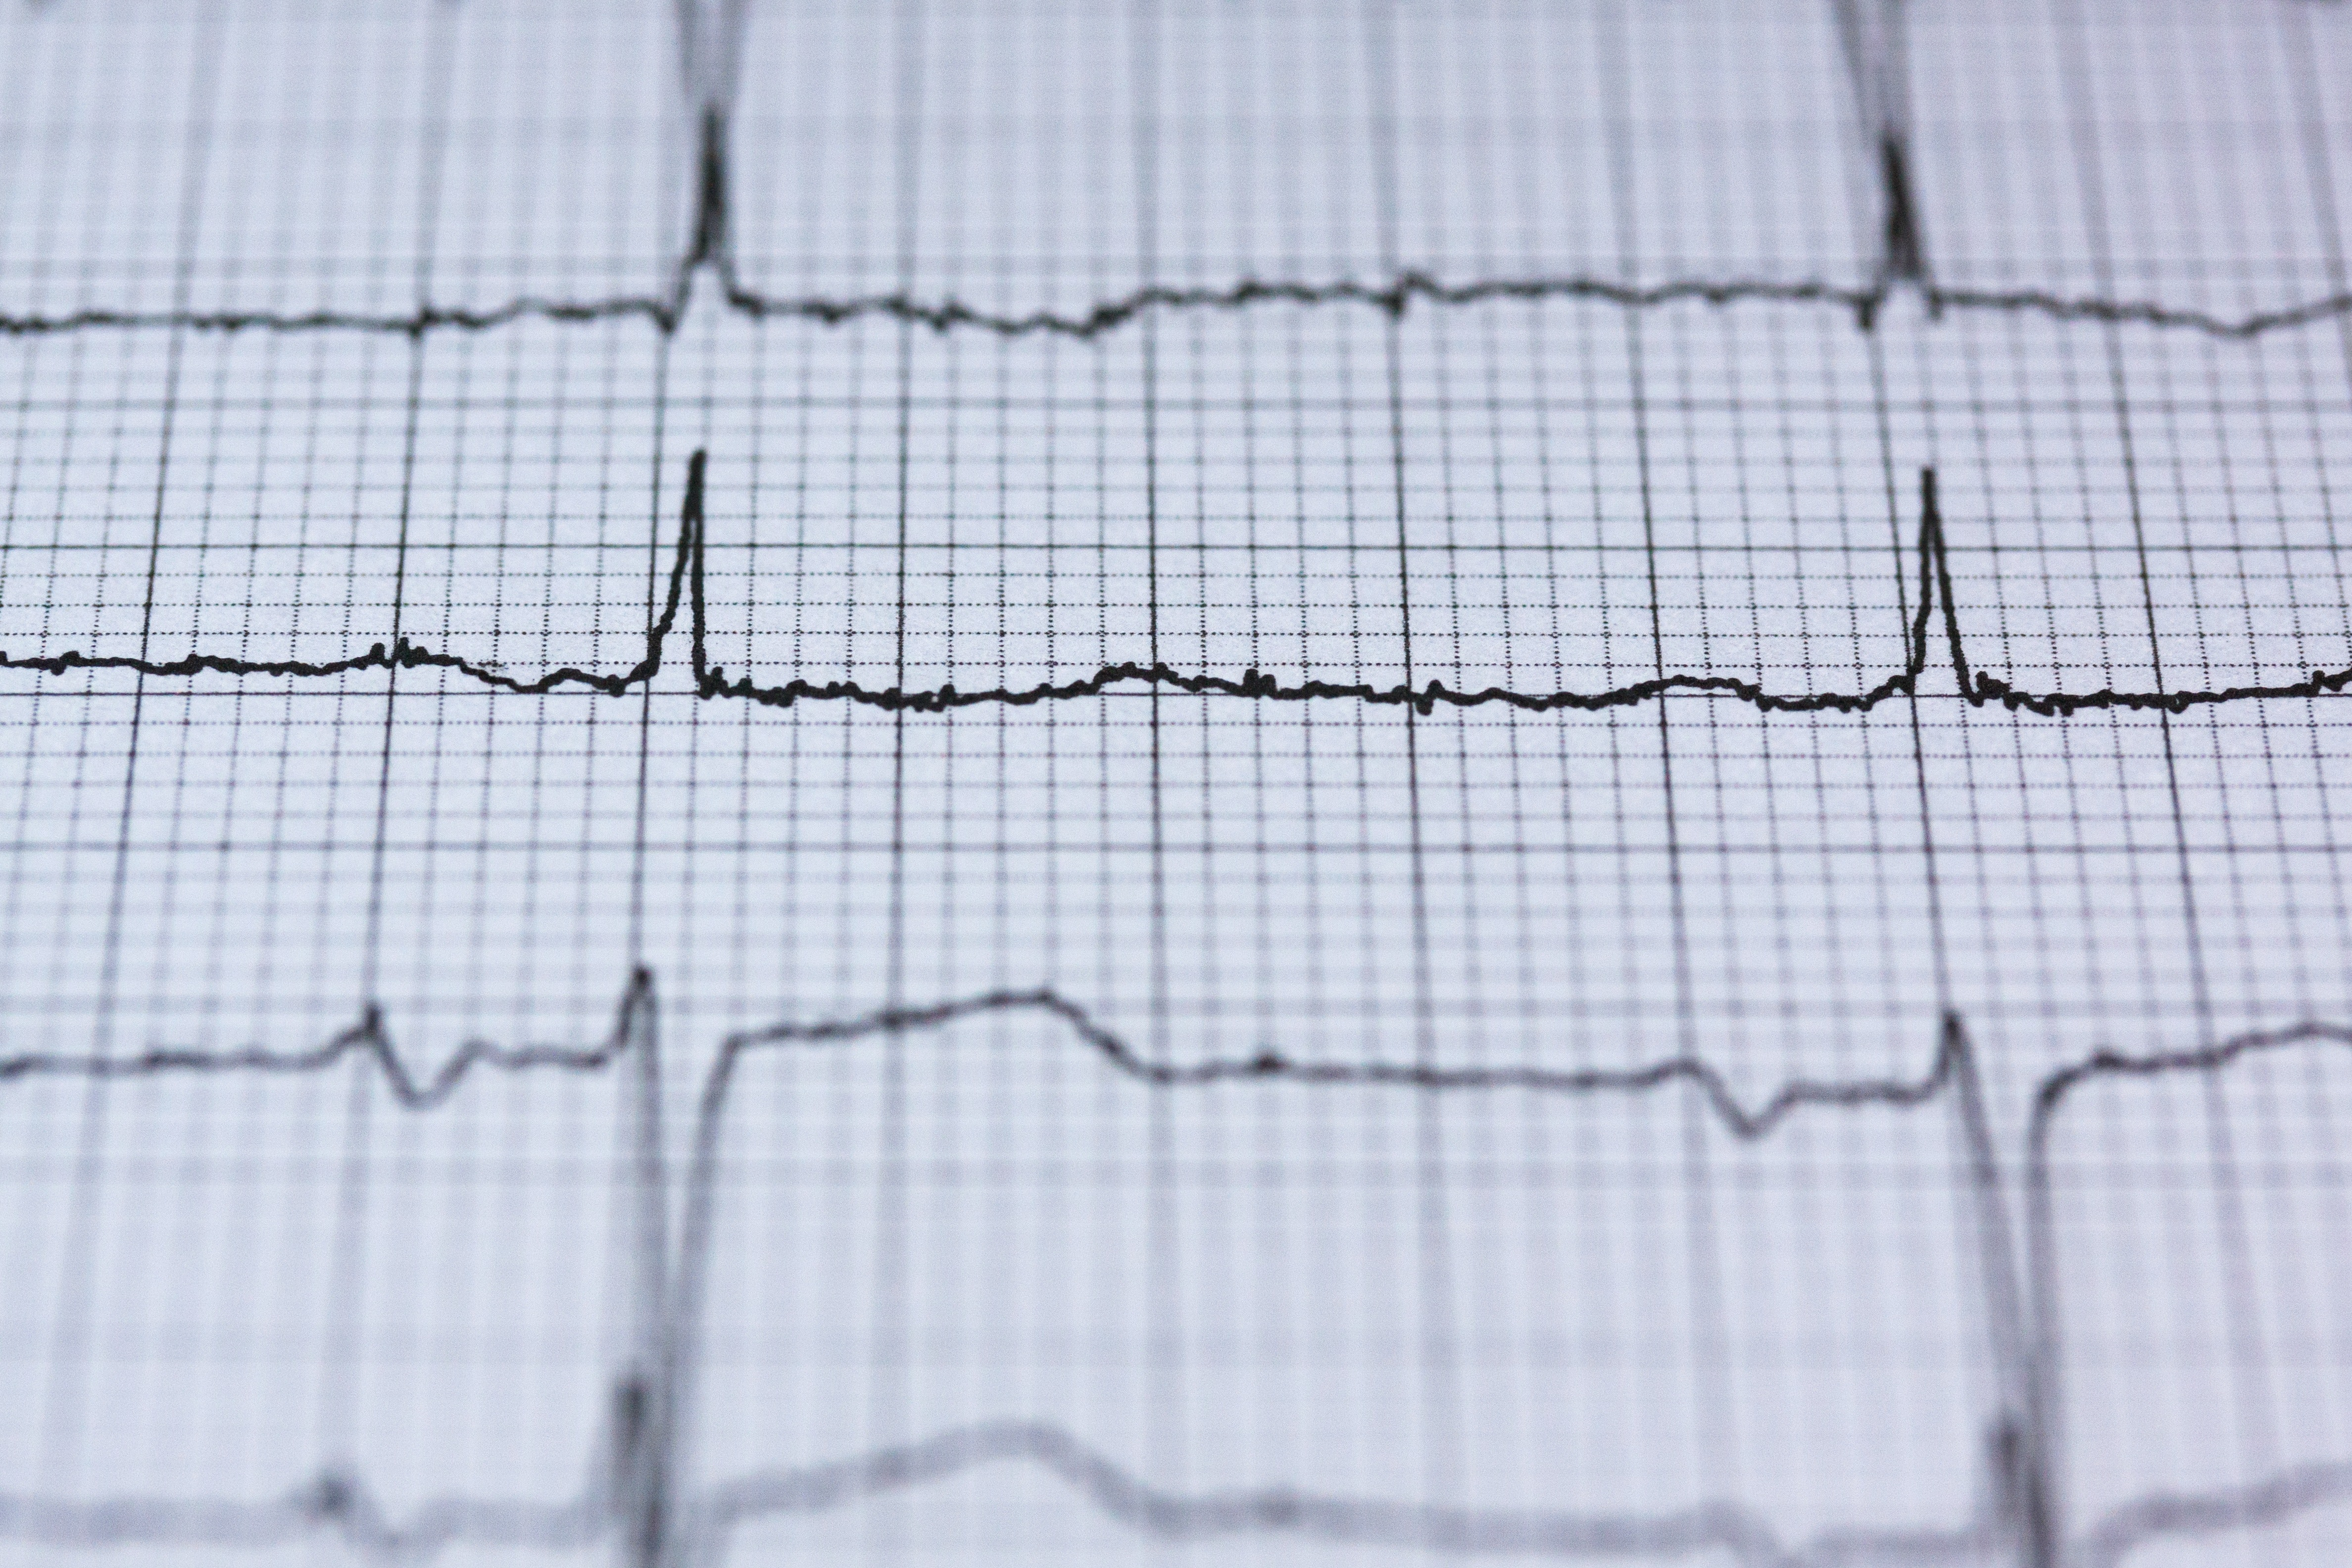
\includegraphics[width=0.45\textwidth, height=0.3\paperheight]{cardiogram.jpg}\\
		\noindent
		\begin{minipage}[t]{0.45\textwidth}
			\begin{itemize}[label=\positiveaspect]
				\item measure nerve impulse \pause
				\item very detailed, reliable \pause
				\item more than BPM \pause
			\end{itemize}
		\end{minipage}
		\hfill\vline\hfill
		\begin{minipage}[t]{0.45\textwidth}
			\begin{itemize}[label=\negativeaspect]
				\item cumbersome manual placement \pause
				\item usually in medical environment \pause
				\item uncomfortable
					
			\end{itemize}
		\end{minipage}
\end{itemize}
\end{frame}

\begin{frame}{Heart rate measurement (Traditional)}
	\begin{itemize}
		\item \mytitle{Photoplethysmography (PPT)}\\
			\vspace{0.2cm}
			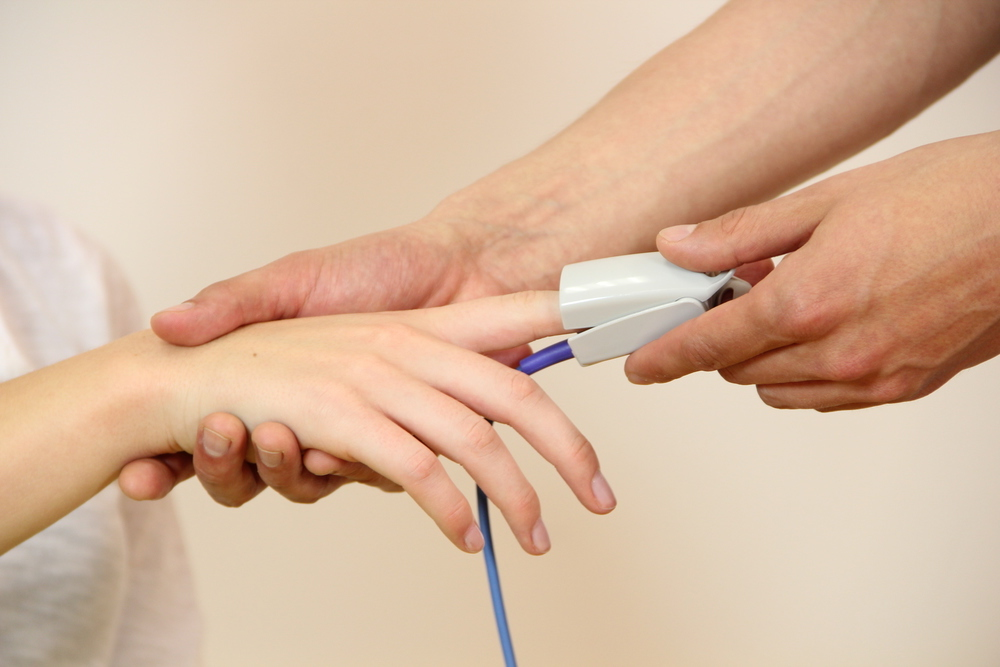
\includegraphics[width=0.45\textwidth, height=0.3\paperheight]{bvp_sensor_mirrored.jpg}
			\hfill
			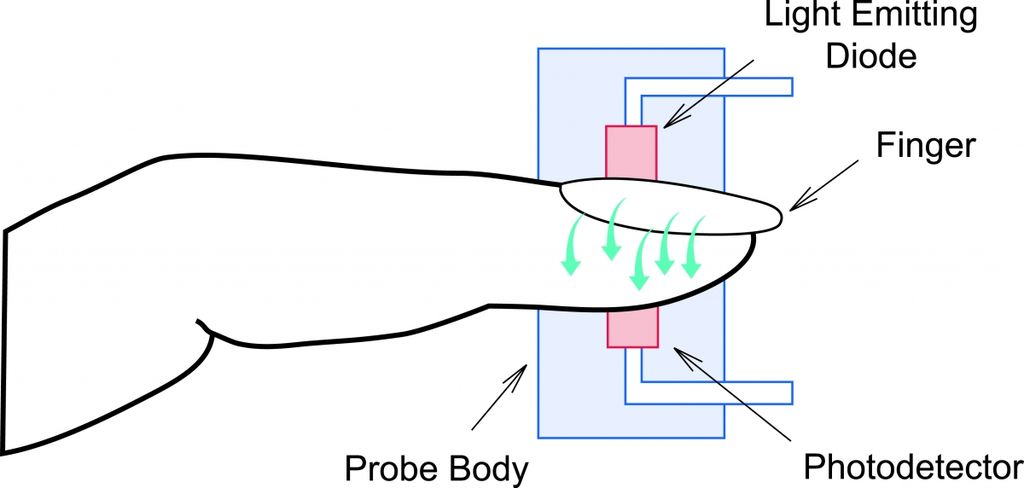
\includegraphics[width=0.45\textwidth, height=0.3\paperheight]{pulse_oximetry_sketch.jpg}\\ \pause
		\noindent
		\begin{minipage}[t]{0.45\textwidth}
			\begin{itemize}[label=\positiveaspect]
				\item fast \pause
				\item uncomplicated \pause
			\end{itemize}
		\end{minipage}
		\hfill\vline\hfill
		\begin{minipage}[t]{0.45\textwidth}
			\begin{itemize}[label=\negativeaspect]
				\item expensive (approx. 250~\$) \pause
				\item uncomfortable over long time
			\end{itemize}
		\end{minipage}
	\end{itemize}
\end{frame}

\begin{frame}{Traditional methods are reliable, but they...}
\pause
	\begin{itemize}[label=\negativeaspect]
		\item ... are expensive. \pause
		\item ... require medical personnel. \pause
		\item ... are uncomfortable for the patient. \pause
	\end{itemize}
	$\Rightarrow$ \textcolor{red}{\textbf{NOT SUITABLE}} for:\\
	\vspace{0.2cm} \pause
	\begin{minipage}[t]{\textwidth}
		\includegraphics[width=0.4\textwidth, align=c]{Sleep-Lab-facilities.jpg}
		\hspace{2cm}
		long time studies
	\end{minipage}\\ \pause
	\begin{minipage}[t]{\textwidth}
		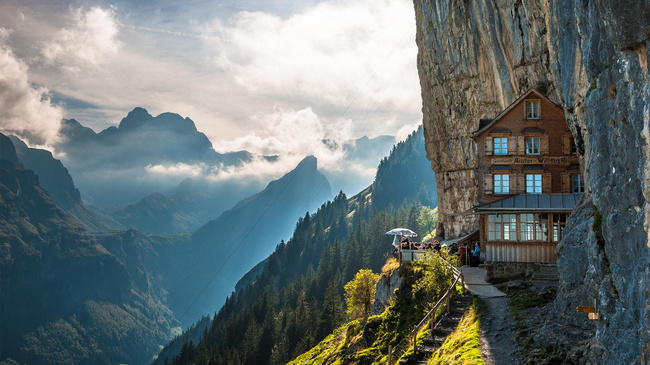
\includegraphics[width=0.4\textwidth, align=c]{berggasthaus_aescher.jpg}
		\hspace{2cm}
		telemedicine
	\end{minipage}
\end{frame}

\begin{frame}{A new hope: Using a camera}
	\begin{minipage}{0.3\textwidth}
		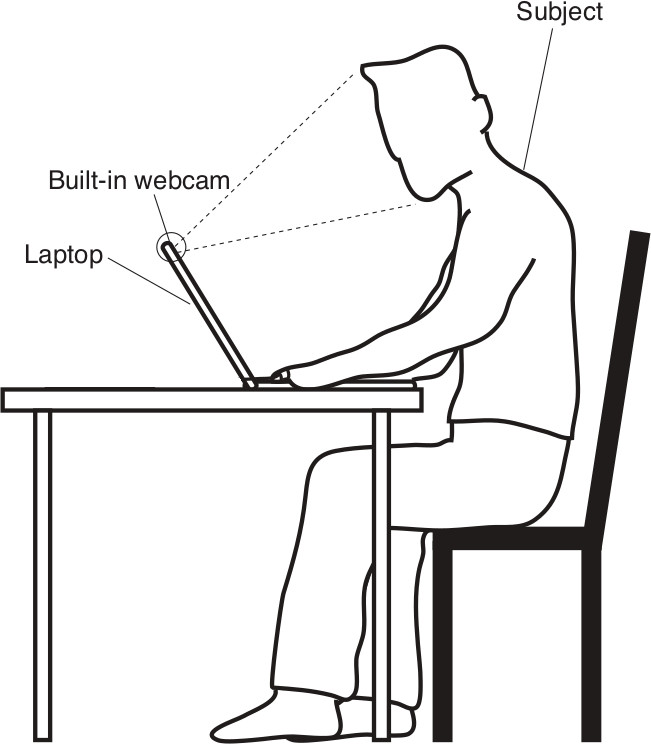
\includegraphics[width=\textwidth]{setup_no_bvp.jpg}
	\end{minipage} \pause
	\hfill
	\begin{minipage}{0.5\textwidth}
		\begin{itemize}[label=\positiveaspect]
			\item very cheap \pause
			\item everybody has a laptop/smartphone \pause
			\item very comfortable \pause
			\item can handle multiple patients at once
		\end{itemize}
	\end{minipage}
\end{frame}

\end{document}